\textit{Amostre o sinal  a um período de amostragem e determine os seguintes:}

\subsubsection*{(a) \textbf{(1,0 pontos) }}
\textit{Calcule a DFT e FFT do sinal amostrado com uma janela de somente 32 amostras. É possível observar no espectro as senóides?}

\begin{figure}[H]
    \centering
    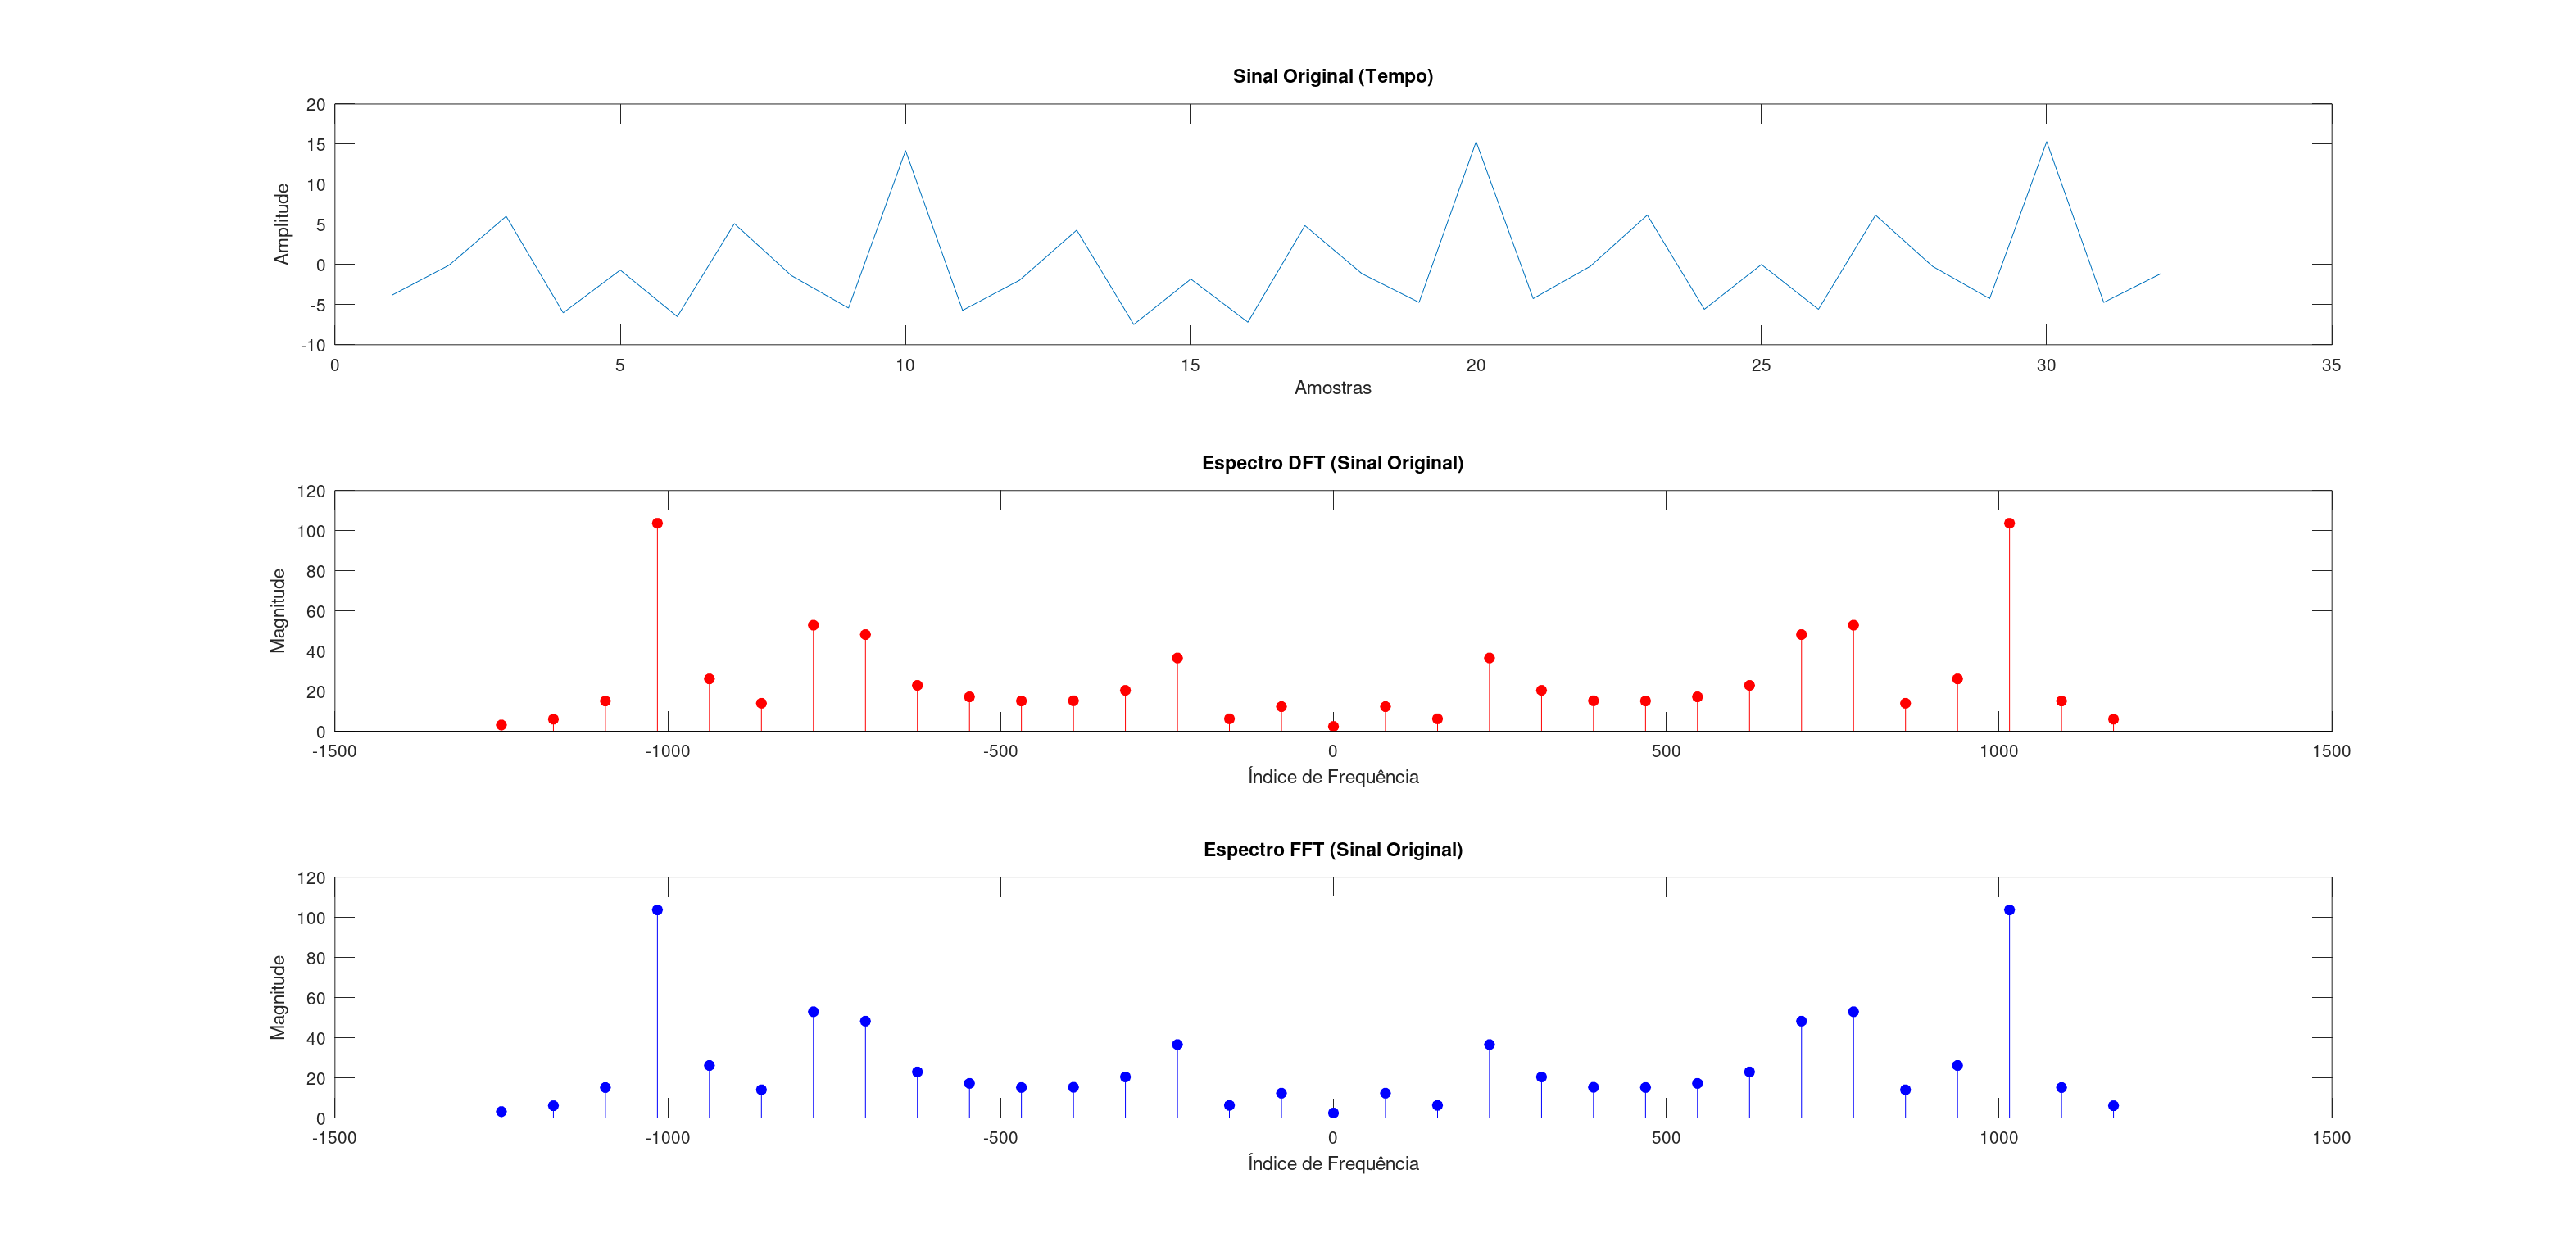
\includegraphics[width=1\linewidth]{03_experimental_analysis//assets/plot_results/32_samples_dft_fft.png}
    \caption{DFT+FFT Aplicada a 32 amostras}
    \label{fig:signal_32samples_fft-dft}
\end{figure}

Realizando a análise a partir da Figura \ref{fig:signal_32samples_fft-dft} é possível observar que, embora o espectro não esteja completamente definido e os picos não sejam perfeitamente nítidos, as senóides aparecem no espectro.

\begin{itemize}
    \item \textbf{Um pico inicial próximo de 100 Hz} indica a presença de uma componente de \textbf{100 Hz}, que corresponde à primeira senóide do sinal.
    \item \textbf{Picos próximos de 250 Hz} indicam uma componente de \textbf{250 Hz}.
    \item \textbf{Picos próximos de 750 Hz} sugerem uma componente de \textbf{750 Hz}.
    \item \textbf{Picos próximos de 1000 Hz} indicam uma componente de \textbf{1000 Hz}.
\end{itemize}

Esses picos no espectro estão alinhados com as senóides presentes no sinal original. Além disso, apesar de haver valores próximos de $500 \, \text{Hz}$, o mesmo se mantém consistente com a ausência de uma componente de $500 \, \text{Hz}$ no sinal.

Apesar de o espectro não apresentar uma definição perfeita e de alguns picos estarem um pouco dispersos, ele ainda confirma a presença das senóides e valida a análise espectral do sinal.

%%%%%%%%%%%%%%%%%%%%%%%%%%%%%%%%%%%%%%%%%%%%%%%%%%%%%%%%%%%%%%%%%%%%%%
\subsubsection*{(b) \textbf{(1,0 pontos)}}
\textit{Aumente o comprimento do item anterior para 64 amostras, aumentando 32 zeros à direita das amostras originais. Calcule a DFT e FFT. Compare com o item anterior e comente seus resultados.}

Através da análise na Figura \ref{fig:signal_32samples_fft-dft_padded}, pode-se observar que quantidade de picos próximos de frequências específicas aumentou com o aumento do número de amostras de 32 para 64.

\begin{figure}[H]
    \centering
    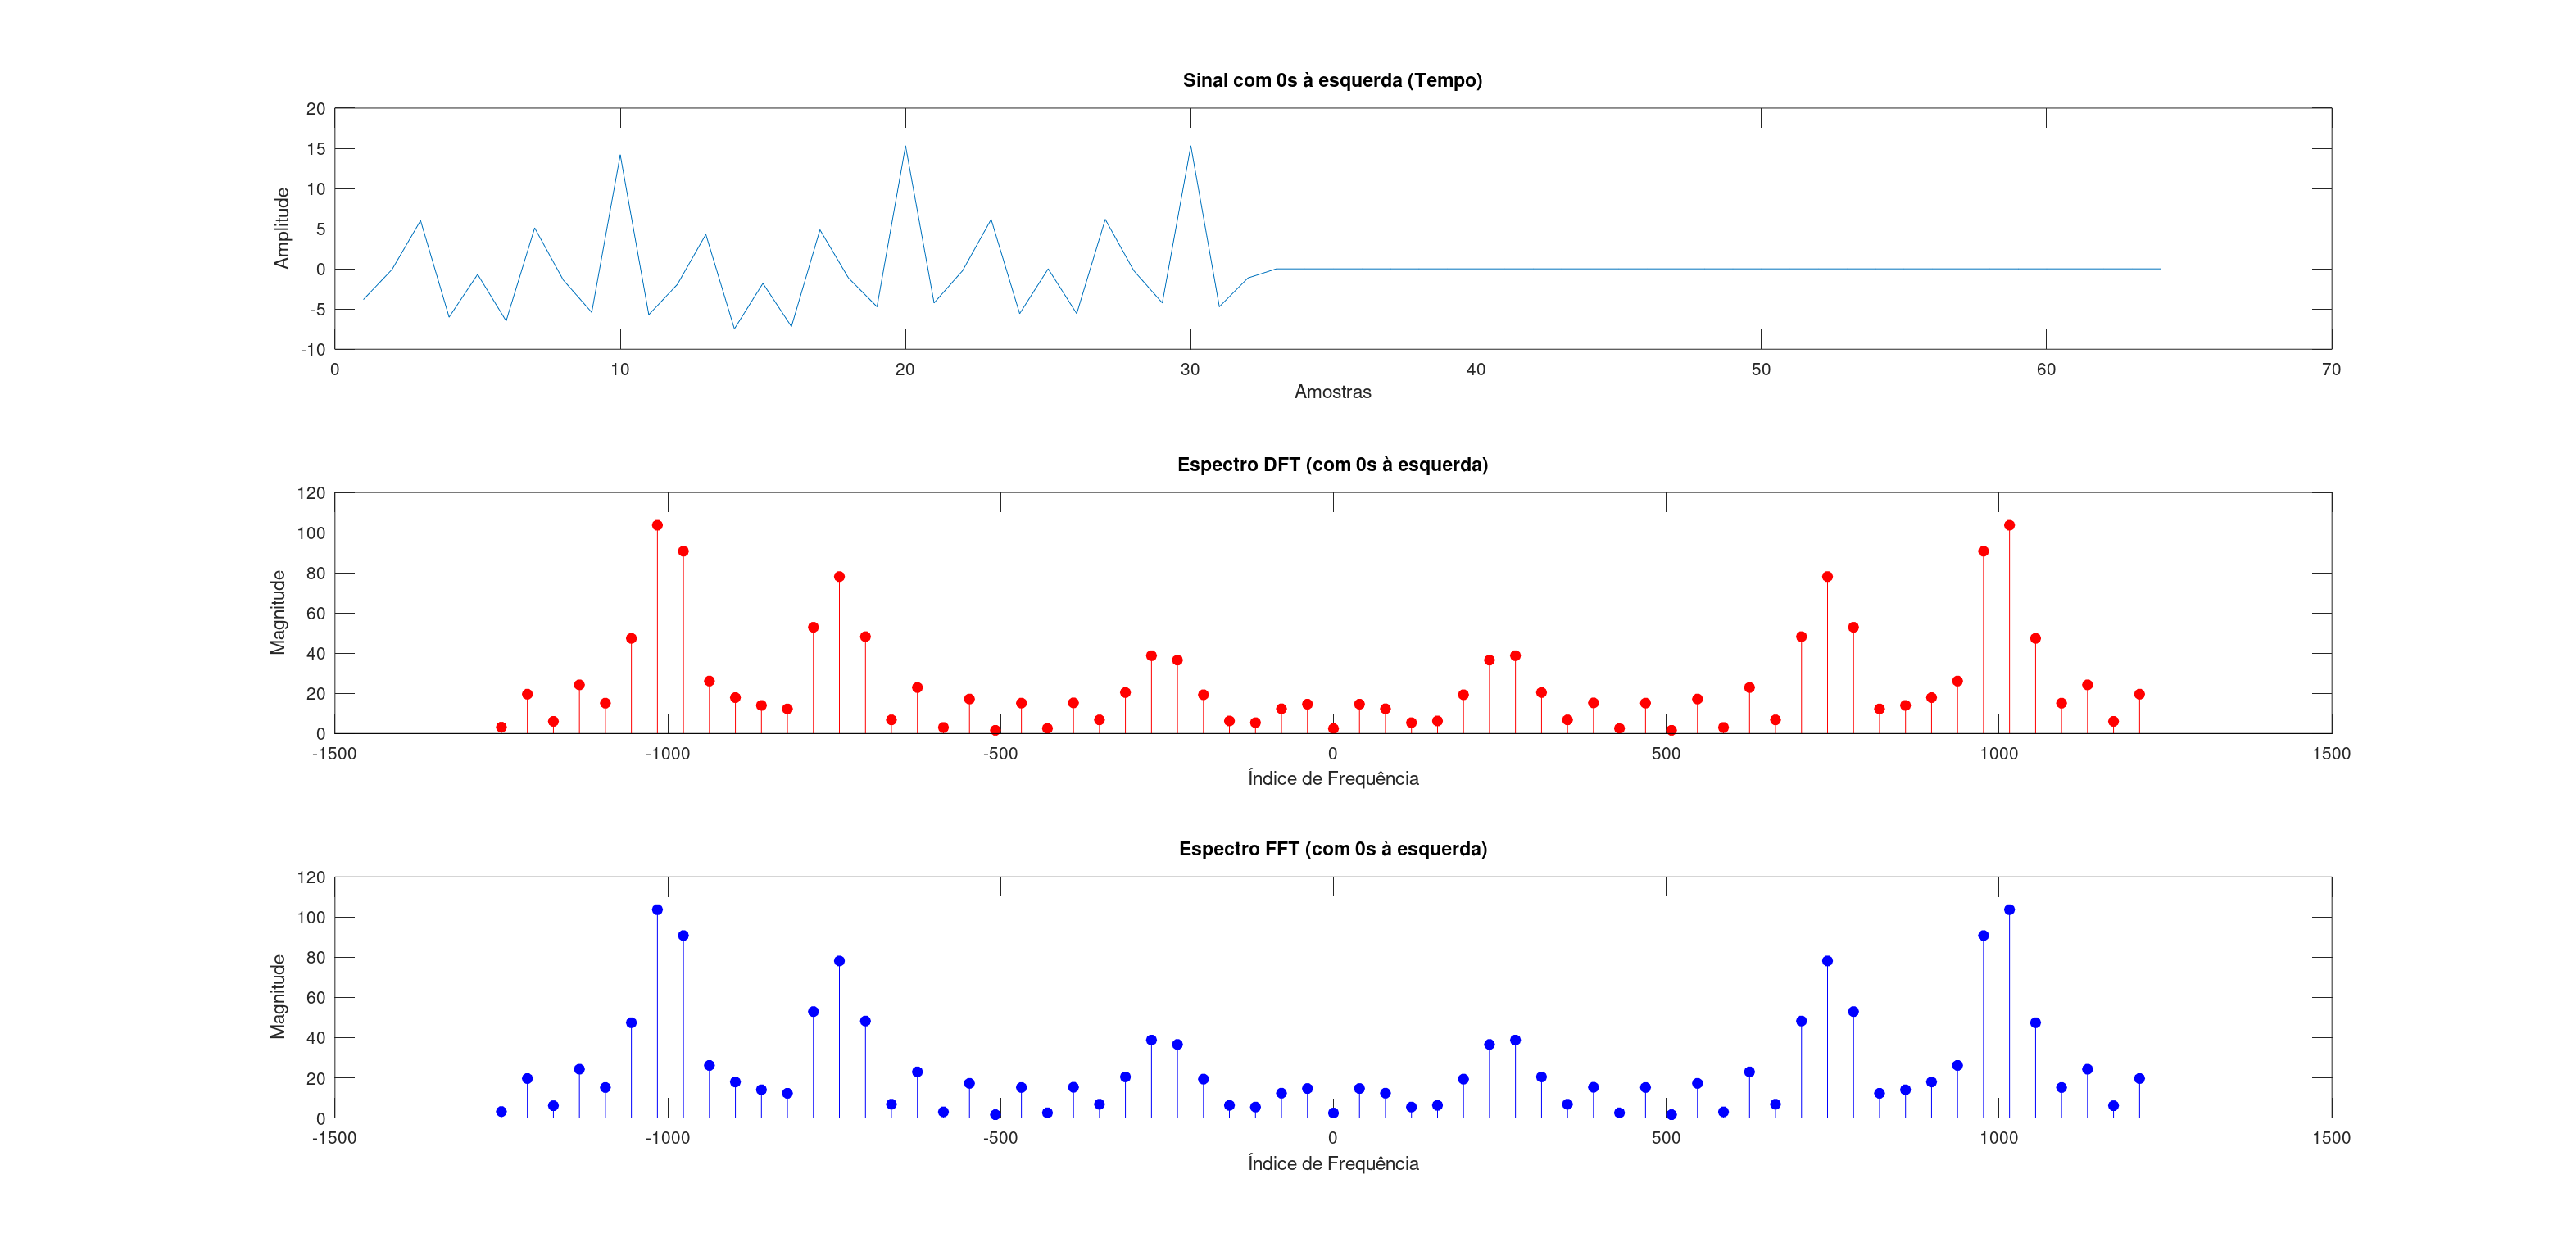
\includegraphics[width=1\linewidth]{03_experimental_analysis//assets/plot_results/32_samples_dft_fft_padded.png}
    \caption{DFT+FFT Aplicada a 32 amostras com 32 zeros à direita}
    \label{fig:signal_32samples_fft-dft_padded}
\end{figure}

Apesar de não adicionar novas informações ao sinal, a inclusão de zeros à direita na sequência de dados, ocasionou no aumento da quantidade de pontos no domínio da frequência.

Como resultado, a DFT ou FFT se torna mais resolvida, o que significa que ela é capaz de identificar mais picos em torno das frequências dominantes. Isso causa um "refinamento" da forma do espectro, revelando picos em frequências mais próximas e aumentando a quantidade de picos visíveis.

%%%%%%%%%%%%%%%%%%%%%%%%%%%%%%%%%%%%%%%%%%%%%%%%%%%%%%%%%%%%%%%%%%%%%%
\subsubsection*{(c) \textbf{(1,0 pontos)}}
\textit{Calcule a DFT e FFT usando uma janela de 64 amostras. É possivel observar no espectro as senóides?}

De forma análoga ao que foi observado anteriromente, ao observar a Figura \ref{fig:signal_64samples_fft-dft}, é possível notar os mesmos picos no espectro que o sinal com 32 zeros à direita.

\begin{figure}[H]
    \centering
    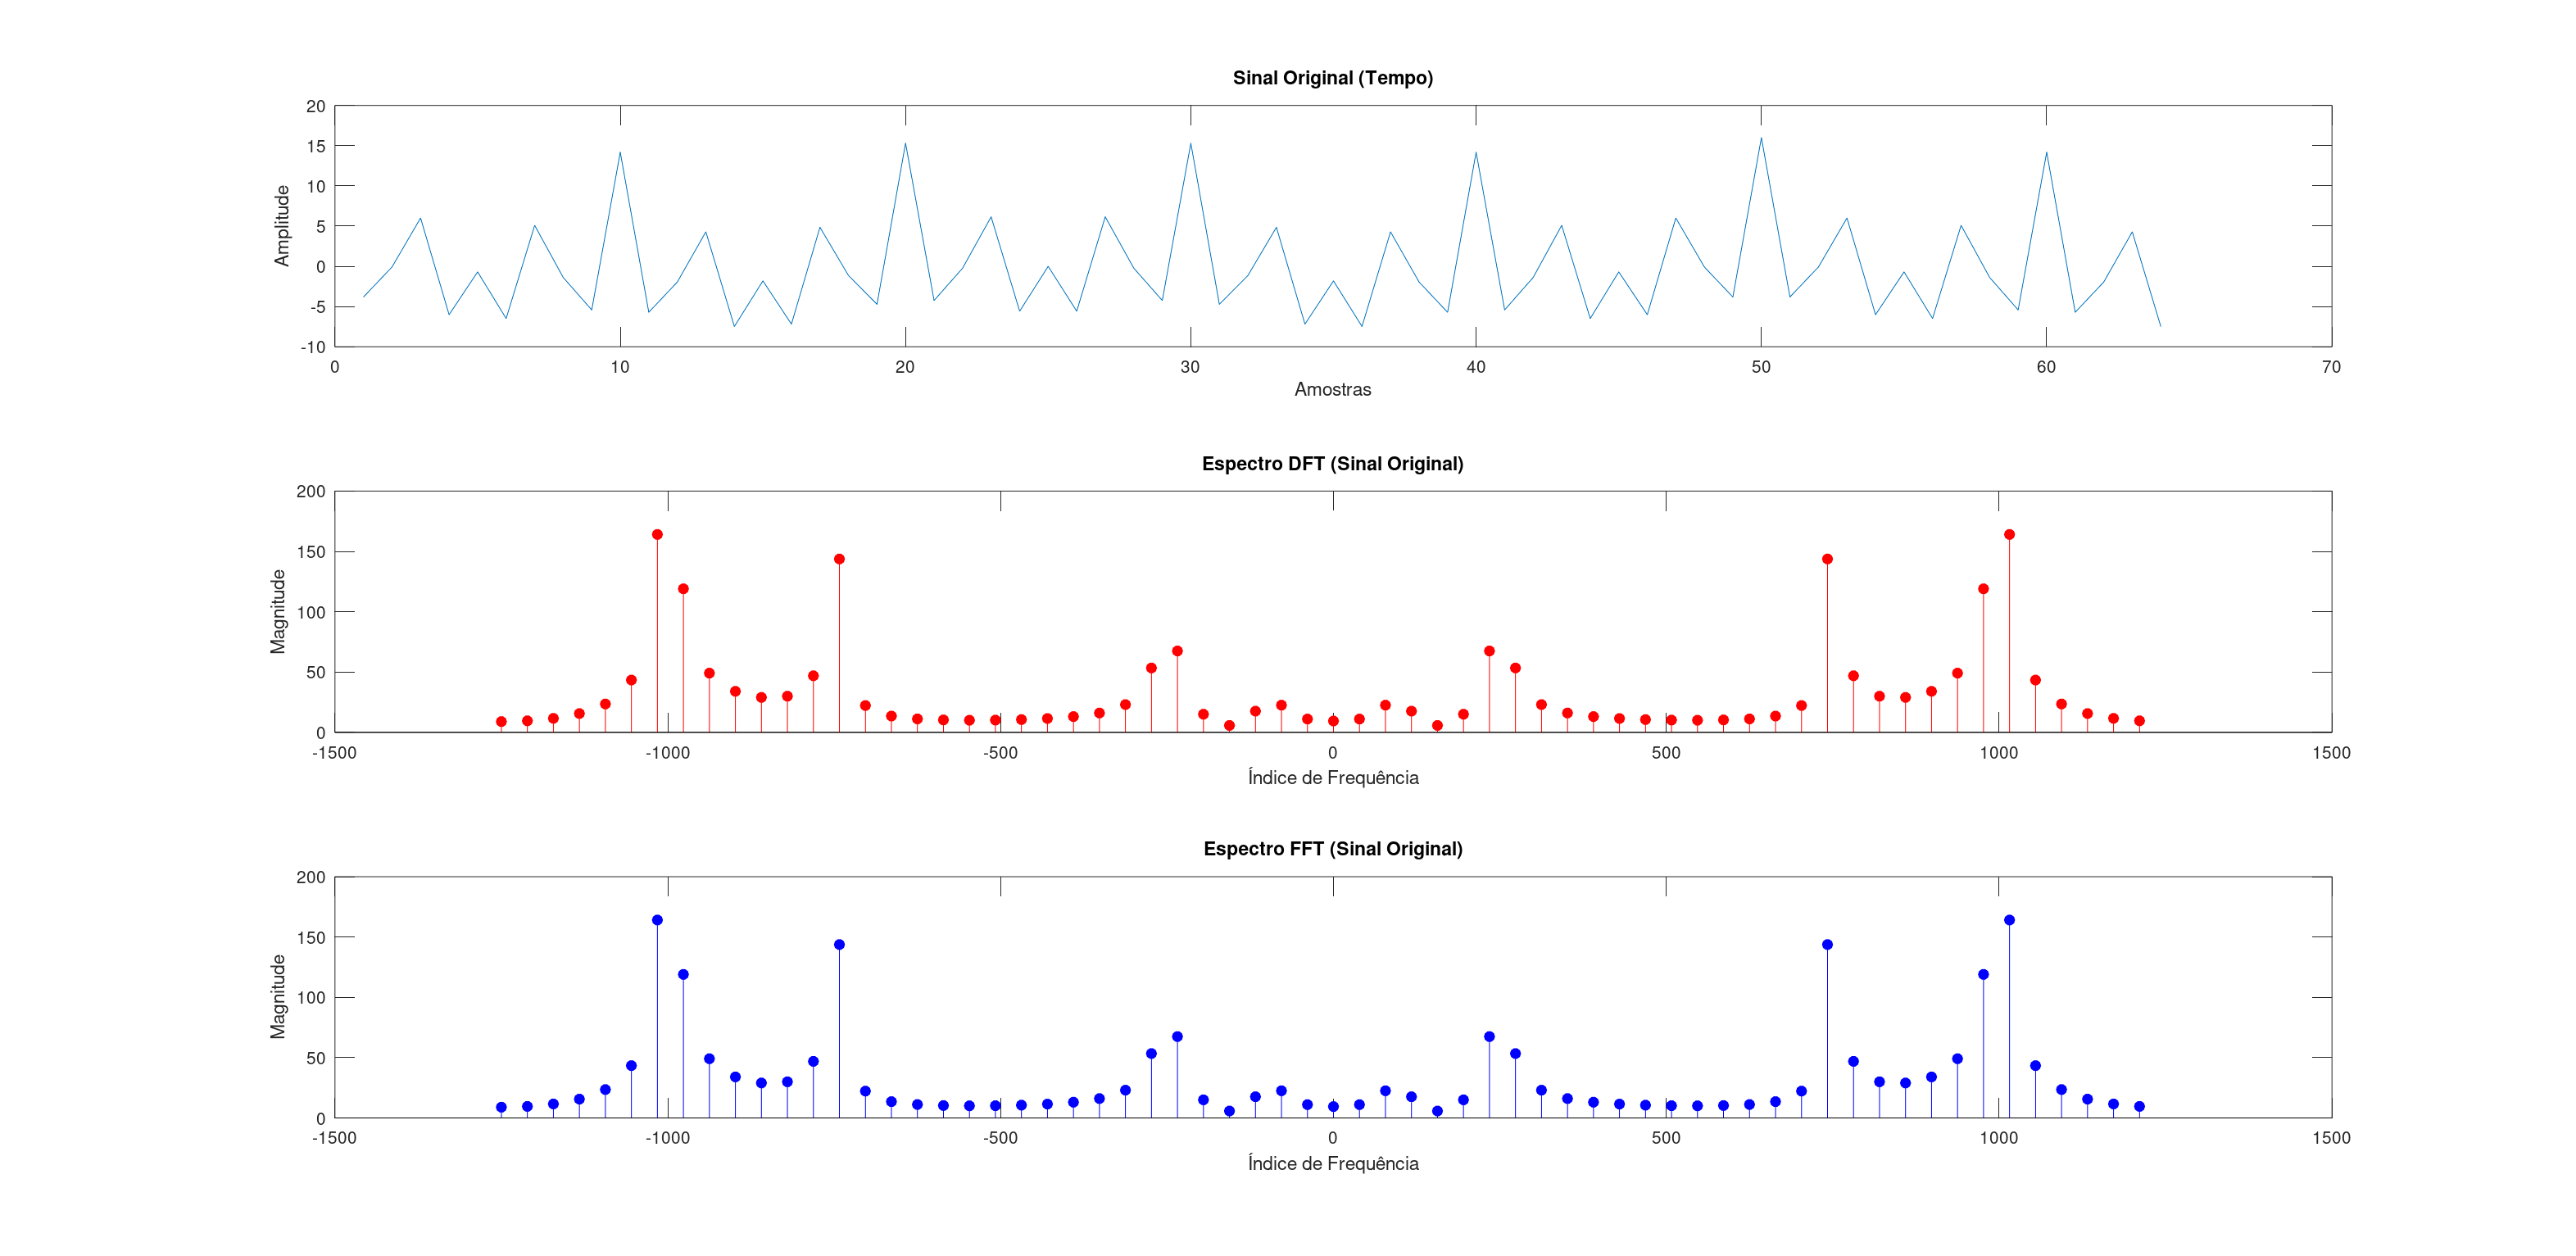
\includegraphics[width=1\linewidth]{03_experimental_analysis//assets/plot_results/64_samples_dft_fft.png}
    \caption{DFT+FFT Aplicada a 64 amostras}
    \label{fig:signal_64samples_fft-dft}
\end{figure}

É importante observar que apesar de ter picos em posições semelhantes, as amplitudes em cada ponto da frequência possui uma variação menor, tornando assim o espectro mais estável e visível.

%%%%%%%%%%%%%%%%%%%%%%%%%%%%%%%%%%%%%%%%%%%%%%%%%%%%%%%%%%%%%%%%%%%%%%
\subsubsection*{(d) \textbf{(1,0 pontos)}}
\textit{Aumente o comprimento do item anterior para 128 amostras, aumentando 64 zeros à direita das amostras originais. Calcule a DFT e FFT. Compare com o item anterior e comente seus resultados.}

Ao observar a Figura \ref{fig:signal_64samples_fft-dft_padded}, podemos observar que há um efeito análogo ao que foi previamente discutido ao aumentar de \textbf{32 para 64 amostras}. Ao incluir mais zeros, o número de pontos no domínio da frequência aumenta, proporcionando uma maior resolução espectral.

\begin{figure}[H]
    \centering
    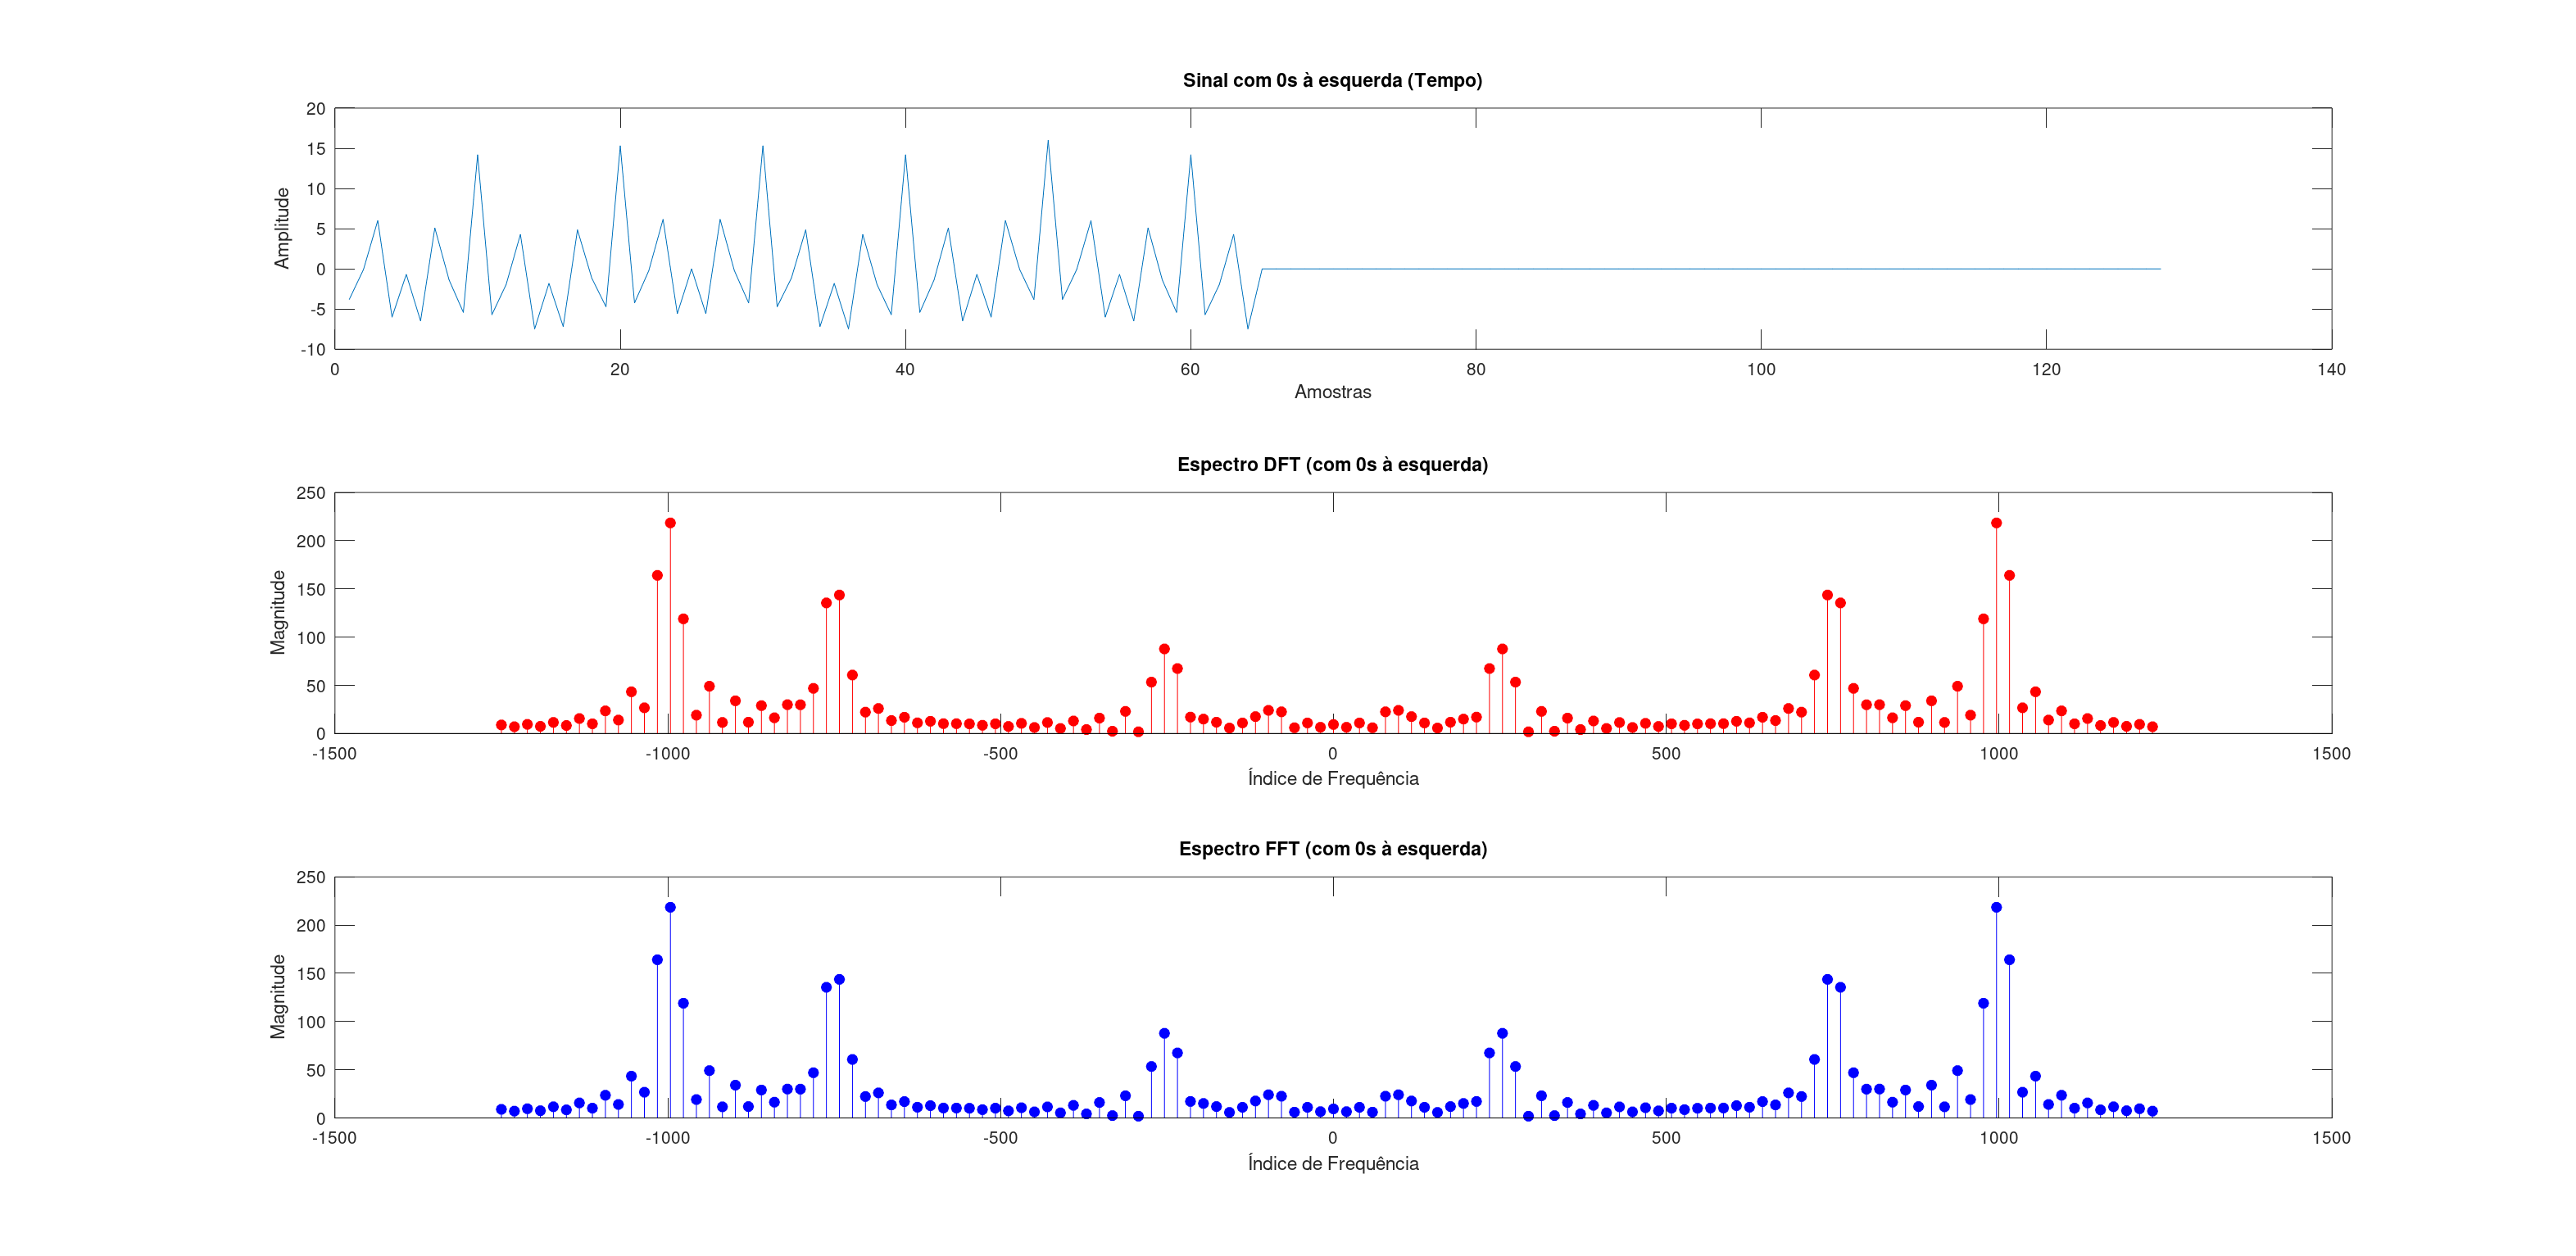
\includegraphics[width=1\linewidth]{03_experimental_analysis//assets/plot_results/64_samples_dft_fft_padded.png}
    \caption{DFT+FFT Aplicada a 64 amostras com 64 zeros à direita}
    \label{fig:signal_64samples_fft-dft_padded}
\end{figure}

Essa melhoria na definição espectral com \textbf{128 amostras} torna mais fácil identificar as frequências componentes, especialmente em sinais que contêm múltiplas componentes próximas, como no caso das senóides de 250 Hz, 750 Hz e 1000 Hz.

%%%%%%%%%%%%%%%%%%%%%%%%%%%%%%%%%%%%%%%%%%%%%%%%%%%%%%%%%%%%%%%%%%%%%%
\subsubsection*{(f) \textbf{(1,0 pontos)}}
Monte numa tabela comparativa a quantidade de operações (produtos e somas) realizadas.

\begin{table}[ht]
    \centering
    \begin{tabular}{lccc}
    \textit{\textbf{Amostras}}            & \textbf{DFT (Ops)} & \textbf{FFT (Sums)} & \textbf{FFT (Mult)} \\
    \textit{32}                       & 1024                                & 160                  & 80                            \\
    \textit{32 + 32 0s}     & 4096                                & 384                  & 192                           \\
    \textit{64}                       & 4096                                & 384                  & 192                           \\
    \textit{64 + 64 0s}     & 16384                               & 896                  & 448                           \\
    \textit{128}                      & 16384                               & 896                  & 448                           \\
    \textit{128 + 128 0s}   & 65536                               & 2048                 & 1024                          \\
    \textit{256}                      & 65536                               & 2048                 & 1024                          \\
    \textit{256 + 256 0s}   & 262144                              & 4608                 & 2304                          \\
    \textit{512}                      & 262144                              & 4608                 & 2304                          \\
    \textit{512 + 512 0s}   & 1048576                             & 10240                & 5120                          \\
    \textit{1024}                     & 1048576                             & 10240                & 5120                          \\
    \textit{1024 + 1024 0s} & 4194304                             & 22528                & 11264                        
    \end{tabular}
    \caption{Comparativo da quantidade de operações (produtos e somas) realizadas em diferentes configurações de amostras.}
    \label{tab:operacoes_comparativo}
\end{table}


\subsubsection*{(f) \textbf{(1,0 pontos)}}
\textit{Monte numa tabela comparativa a quantidade de operações (produtos e somas) realizadas.}

Baseando-se no resultado obtido a partir da execução dos algoritmos, foi construída a tabela \ref{tab:operacoes_comparativo}, que apresenta o número de operações necessárias para calcular as transformadas de Fourier discreta (DFT) e rápida (FFT) para diferentes tamanhos de amostra.

\begin{table}[ht]
    \centering
    \begin{tabular}{lccc}
    \textit{\textbf{Amostras}}            & \textbf{DFT (Ops)} & \textbf{FFT (Sums)} & \textbf{FFT (Mult)} \\
    \textit{32}                       & 1024                                & 160                  & 80                            \\
    \textit{32 + 32 0s}     & 4096                                & 384                  & 192                           \\
    \textit{64}                       & 4096                                & 384                  & 192                           \\
    \textit{64 + 64 0s}     & 16384                               & 896                  & 448                           \\
    \textit{128}                      & 16384                               & 896                  & 448                           \\
    \textit{128 + 128 0s}   & 65536                               & 2048                 & 1024                          \\
    \textit{256}                      & 65536                               & 2048                 & 1024                          \\
    \textit{256 + 256 0s}   & 262144                              & 4608                 & 2304                          \\
    \textit{512}                      & 262144                              & 4608                 & 2304                          \\
    \textit{512 + 512 0s}   & 1048576                             & 10240                & 5120                          \\
    \textit{1024}                     & 1048576                             & 10240                & 5120                          \\
    \textit{1024 + 1024 0s} & 4194304                             & 22528                & 11264                        
    \end{tabular}
    \caption{Comparativo da quantidade de operações (produtos e somas) realizadas em diferentes configurações de amostras.}
    \label{tab:operacoes_comparativo}
\end{table}


Baseando-se na Tabela \ref{tab:operacoes_comparativo}, foi realizo o plot dos seus valores na figura Figura \ref{fig:operations_comparison_graph}. Os resultados demonstram que a FFT é significativamente mais eficiente do que a DFT em termos de complexidade computacional, especialmente para grandes tamanhos de amostra.

\begin{figure}[H]
    \centering
    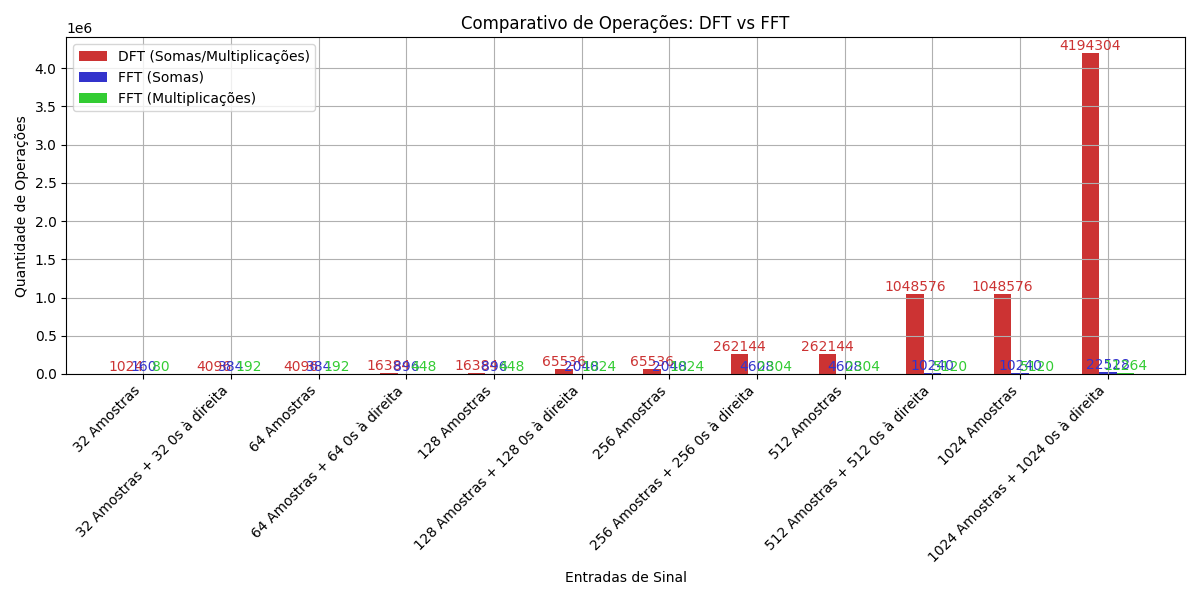
\includegraphics[width=1\linewidth]{03_experimental_analysis//assets/operations_comparison.png}
    \caption{Gráfico comparativo entre a quantidade de operações dos resultados}
    \label{fig:operations_comparison_graph}
\end{figure}

O comportamento do gráfico deixa claro as características do algoritmos, pois enquanto a DFT possui uma complexidade $O(N^2)$, a FFT possui a complexidade $O(N\log{N})$.

À medida que o número de amostras aumenta, a quantidade de operações cresce, mas a FFT realiza muito menos operações que a DFT, destacando sua maior eficiência. Apesar da diferença inicial, para as amostras pequenas (como 32), ser de cerca de 6.4x, essa diferença se torna cada vez mais significativa para amostras maiores.

Portanto, é possível observar que a FFT apresenta um crescimento mais suave nas operações de soma e multiplicação em comparação com a DFT.

